%%
%% This is file `sample-authordraft.tex',
%% generated with the docstrip utility.
%%
%% The original source files were:
%%
%% samples.dtx  (with options: `authordraft')
%% 
%% IMPORTANT NOTICE:
%% 
%% For the copyright see the source file.
%% 
%% Any modified versions of this file must be renamed
%% with new filenames distinct from sample-authordraft.tex.
%% 
%% For distribution of the original source see the terms
%% for copying and modification in the file samples.dtx.
%% 
%% This generated file may be distributed as long as the
%% original source files, as listed above, are part of the
%% same distribution. (The sources need not necessarily be
%% in the same archive or directory.)
%%
%% The first command in your LaTeX source must be the \documentclass command.
\documentclass[sigconf]{acmart}
%% NOTE that a single column version may required for 
%% submission and peer review. This can be done by changing
%% the \doucmentclass[...]{acmart} in this template to 
%% \documentclass[manuscript,screen]{acmart}
%% 
%% To ensure 100% compatibility, please check the white list of
%% approved LaTeX packages to be used with the Master Article Template at
%% https://www.acm.org/publications/taps/whitelist-of-latex-packages 
%% before creating your document. The white list page provides 
%% information on how to submit additional LaTeX packages for 
%% review and adoption.
%% Fonts used in the template cannot be substituted; margin 
%% adjustments are not allowed.

%%
%% \BibTeX command to typeset BibTeX logo in the docs
\AtBeginDocument{%
  \providecommand\BibTeX{{%
    \normalfont B\kern-0.5em{\scshape i\kern-0.25em b}\kern-0.8em\TeX}}}

%% Rights management information.  This information is sent to you
%% when you complete the rights form.  These commands have SAMPLE
%% values in them; it is your responsibility as an author to replace
%% the commands and values with those provided to you when you
%% complete the rights form.
%\setcopyright{acmcopyright}
%\copyrightyear{2021}
%\acmYear{2021}
%\acmDOI{10.1145/1122445.1122456}

%% These commands are for a PROCEEDINGS abstract or paper.
%\acmConference[CS573 Fall '21]{CS573 Fall '21: Data Mining}{August 23--December 08, 2021}{Purdue University, IN}
%\acmBooktitle{CS573 Fall '21: Final Project Proposal,
%  September 26, 2021, Purdue University, IN}
%\acmPrice{15.00}
%\acmISBN{978-1-4503-XXXX-X/18/06}


%%
%% Submission ID.
%% Use this when submitting an article to a sponsored event. You'll
%% receive a unique submission ID from the organizers
%% of the event, and this ID should be used as the parameter to this command.
%%\acmSubmissionID{123-A56-BU3}

%%
%% The majority of ACM publications use numbered citations and
%% references.  The command \citestyle{authoryear} switches to the
%% "author year" style.
%%
%% If you are preparing content for an event
%% sponsored by ACM SIGGRAPH, you must use the "author year" style of
%% citations and references.
%% Uncommenting
%% the next command will enable that style.
%%\citestyle{acmauthoryear}

%%
%% end of the preamble, start of the body of the document source.
\begin{document}

%%
%% The "title" command has an optional parameter,
%% allowing the author to define a "short title" to be used in page headers.
\title{%
  Final Report \\
  \large CS 573 - Data Mining - Fall 2021}

%%
%% The "author" command and its associated commands are used to define
%% the authors and their affiliations.
%% Of note is the shared affiliation of the first two authors, and the
%% "authornote" and "authornotemark" commands
%% used to denote shared contribution to the research.
\author{Reece Jones}
\affiliation{%
    \institution{Purdue University}
    \country{United States}}
\email{jone1926@purdue.edu}

\author{Eli Silkov}
\affiliation{%
    \institution{Purdue University}
    \country{United States}}
\email{esilkov@purdue.edu}

\author{Nathan Merz}
\affiliation{%
    \institution{Purdue University}
    \country{United States}}
\email{merzn@purdue.edu}

\author{Patrick Li}
\affiliation{%
    \institution{Purdue University}
    \country{United States}}
\email{li3992@purdue.edu}

\author{Varun Vora}
\affiliation{%
    \institution{Purdue University}
    \country{United States}}
\email{vora18@purdue.edu}

%%
%% By default, the full list of authors will be used in the page
%% headers. Often, this list is too long, and will overlap
%% other information printed in the page headers. This command allows
%% the author to define a more concise list
%% of authors' names for this purpose.
\renewcommand{\shortauthors}{Jones, Silkov, Merz, Li, Vora}

%%
%% The abstract is a short summary of the work to be presented in the
%% article.
\begin{abstract}
TODO
\end{abstract}

%%
%% The code below is generated by the tool at http://dl.acm.org/ccs.cfm.
%% Please copy and paste the code instead of the example below.
%%
\begin{CCSXML}
<ccs2012>
   <concept>
       <concept_id>10010147.10010257</concept_id>
       <concept_desc>Computing methodologies~Machine learning</concept_desc>
       <concept_significance>500</concept_significance>
       </concept>
 </ccs2012>
\end{CCSXML}

\ccsdesc[500]{Computing methodologies~Machine learning}

%%
%% Keywords. The author(s) should pick words that accurately describe
%% the work being presented. Separate the keywords with commas.
\keywords{datasets, CS573, food, recipes, machine learning, analysis, visualization, project, group}

%%
%% This command processes the author and affiliation and title
%% information and builds the first part of the formatted document.
\maketitle

\section{Introduction}
Chefs currently must spend a great deal of time and error experimenting with combinations to develop new recipes and many common dishes are a variant on traditional recipes. Providing a better starting point for the development of new recipes would save chefs time experimenting and provide consumers more food variety. It is also important for new, more environmentally-friendly ingredients such as plant-based meat alternatives that do not have as many traditional recipes. Beyond cooking, understanding recipes is important for grocers as understanding which items are often purchased together (as the ingredients for recipes are) allows them to optimize store placement and advertising.

Thus, we chose to apply data mining principles and practices to food recipes. For this topic we conducted a literature review, performed exploratory data analysis, learned models, and created applied outcomes using the learned models, knowledge gained from the literature review, and principles learned from this course. The models seek to predict metadata attributes of recipes, and generate new novel recipes. The applied outcomes apply concepts learned in the course and knowledge gained from the literature review to show a practical use of machine learning with respect to the topic of food recipes.

\section{Dataset}
The dataset we used is the food.com recipe\cite{FoodComRecipe}, provided by Shuyang Li et al. via Kaggle. This dataset contains recipe metadata including time to prepare, nutrition, rating, as well as recipe data such as ingredients and steps.

\subsection{Exploratory Data Analysis}
To better understand the data set for modelling purposes, the group explored the distribution of and correlations between features in the data set. The distribution of ingredients and title keywords are highly concentrated. Out of 9005 ingredients, the top 100 ingredients represent 33\% of the ingredient frequency. The top 100 keywords represent 49\% of the cumulative keyword frequency. 

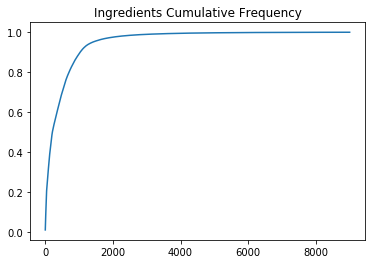
\includegraphics[width=\linewidth]{ingfreq.png}


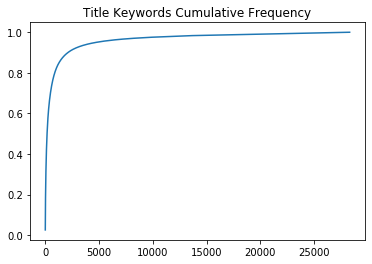
\includegraphics[width=\linewidth]{titfreq.png}

For preparation time, outliers outside the 5-th and 95-th percentiles are capped at the respective percentile. After outlier removal, numerical features still exhibited significant skew. Preparation time and number of steps are skewed right, and rating is skewed left. 73\% of recipes have a preparation time of under 1 hour, and 76\% of recipes have 12 steps or less. 84\% of recipes have an average rating of 4.0 stars or greater. This is something to note for modelling purposes, given that predicting rating  and preparation time are two of the group's goals. The group also examined correlations between numerical features. There is a significant correlation (r=0.43) between the number of steps and number of ingredients. Carbohydrate is negatively correlated with protein and fat content. There are no other significant correlations. Surprisingly, correlation between preparation time and the number of steps is low (r=0.10). 

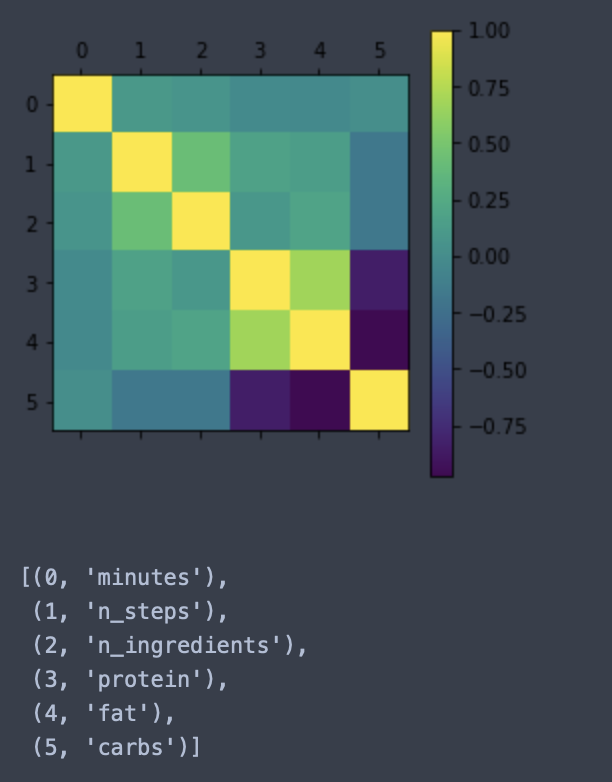
\includegraphics[width=\linewidth]{corrplot.png}

While the group is not using the recipe date as a feature in any models, examining variability of attributes over time yielded two interesting observations. Over the last 3 years, the proportion of fat and protein in recipes has increased. The mean number of steps and preparation time has increased as well.

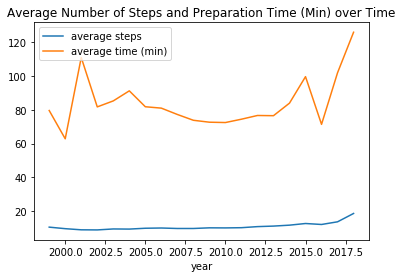
\includegraphics[width=\linewidth]{time_series.png}



\section{Methodology}
We divided our project into multiple tasks: recipe rating prediction, recipe nutrition (calories) prediction, recipe recommendation, recipe ingredient prediction, and recipe generation. For these tasks we used SKLearn, LightGBM, and NLTK for feature extraction and modeling. We discuss our methodologies for each tasks in the following sections.
\subsection{Recipe Rating Prediction}
Rating prediction is a common task of recommender systems, and is accomplished through various collaborative and content-based filtering methods. Because user review data is limited (average of 5 reviews per user), predicting rating of a user given this data set is challenging, and the group decided to attempt to predict the average rating of recipes using available recipe attributes. Ahuja et. al. \cite{RPKmeans} demonstrate the effectiveness of a K-Nearest Neighbors approach in rating prediction. Numerical features used as predictors were preparation time, number of steps, the number of ingredients, and the caloric content decomposed into protein, fat and carbohydrates. 

Additionally, 100 features were generated from text data pertaining to ingredients and the recipe title. A feature was created for each of the top 50 ingredients in the dataset (value of 1 if the ingredient is in the recipe, and 0 if the ingredient is not included in the recipe). A similar feature was created for each of the top 50 recipe title keywords. Given that only title keywords were considered, term frequency was not evaluated. All predictors were scaled to values between 0 and 1. The average rating was rounded to the nearest integer to create 6 discrete ratings classes \{0, 1, ..., 5\}. While cosine similarity if often preferred as a distance metric for rating and recommendation systems, Schwarz et. al. demonstrate that a Euclidean Distance-based approach may be more accurate \cite{RPSimilarity}. Furthermore, given that cosine similarity is most useful when term frequencies differ across documents, and the frequency term is not reflected in the features created, cosine similarity was not used as a distance metric in the K-Nearest Neighbors algorithm.

The K-Nearest Neighbors algorithm was evaluated using L2-distance with a search space of [2, 4, 8, 16, 32, 64, 128, 256, 512] neighbors. Graph below illustrates that the learning curve saturates rapidly.

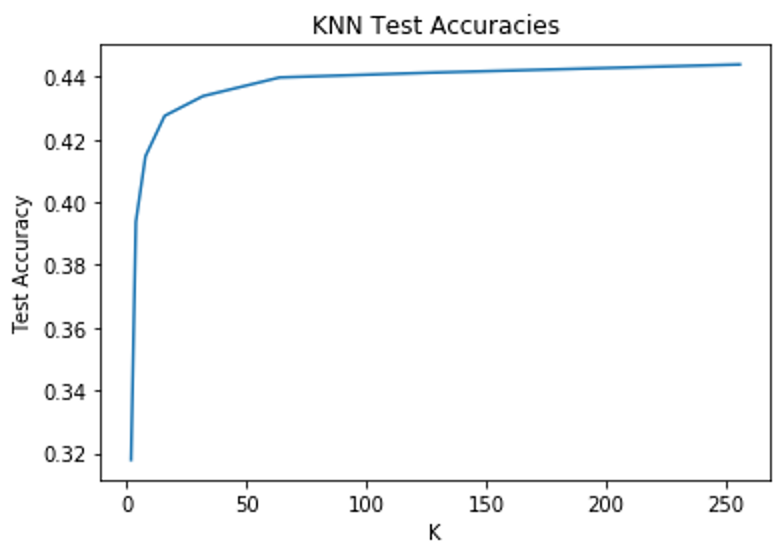
\includegraphics[width=\linewidth]{knnlearningcurve.png}
\captionof{figure}{K-Nearest Neighbors using L2-norm for distance ordering}

Based on the learning curve, a value of K=64 clusters was selected. Performance of the model is poor, with an accuracy of 0.44 using predictions on test data. Jain et. al. demonstrate that when training K-nearest neighbors recommendation and rating algorithms using sparse text data, Manhattan distance (L1 norm) performs better than Euclidean distance / cosine similarity. \cite{RPL1Norm}. Given that the vectors for ingredients and title keywords are sparse, a L1 norm K Nearest Neighbors approach was implemented as well. 

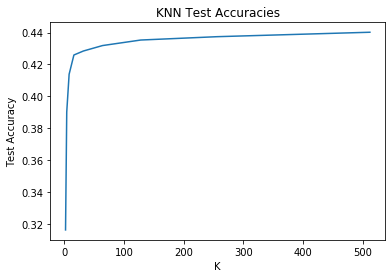
\includegraphics[width=\linewidth]{l1norm.png}
\captionof{figure}{K-Nearest Neighbors using L1-norm for distance ordering}

Accuracy of an L1-norm K-Nearest Neighbors approach yielded no improvement versus the L2-norm approach. Given poor model performance, alternative modelling techniques were explored. These included linear regression, Naive Bayes Classifier and K-Nearest Neighbors using only numerical attributes. All of these methodologies performed worse than the initial K-Nearest Neighbors approach. 


\subsection{Recipe Nutrition Prediction}
The task of Recipe Nutrition Prediction, specifically that of predicting calorie values, was accomplished using a decision tree. Calorie values were chosen due to their being ubiquitous in everyday life and also intuitively being probably more correlated with the other attributes than something like sodium content. The tree was trained on the attributes of recipe time in minutes, recipe number of ingredients, and recipe number of steps. With the exception of date(which did not have a major effect on the other attributes as seen in the data analysis), this covered all continuous features that were not directly nutrition related. To aid computation speed, all features were discretized into 2 quantiles. Due to the significant right skew found on many attributes such as recipe time and calorie level, discretization into equal sized bins is highly unsuitable for this step. Gini gain was used as the splitting measure with an 80/20 train/test split.
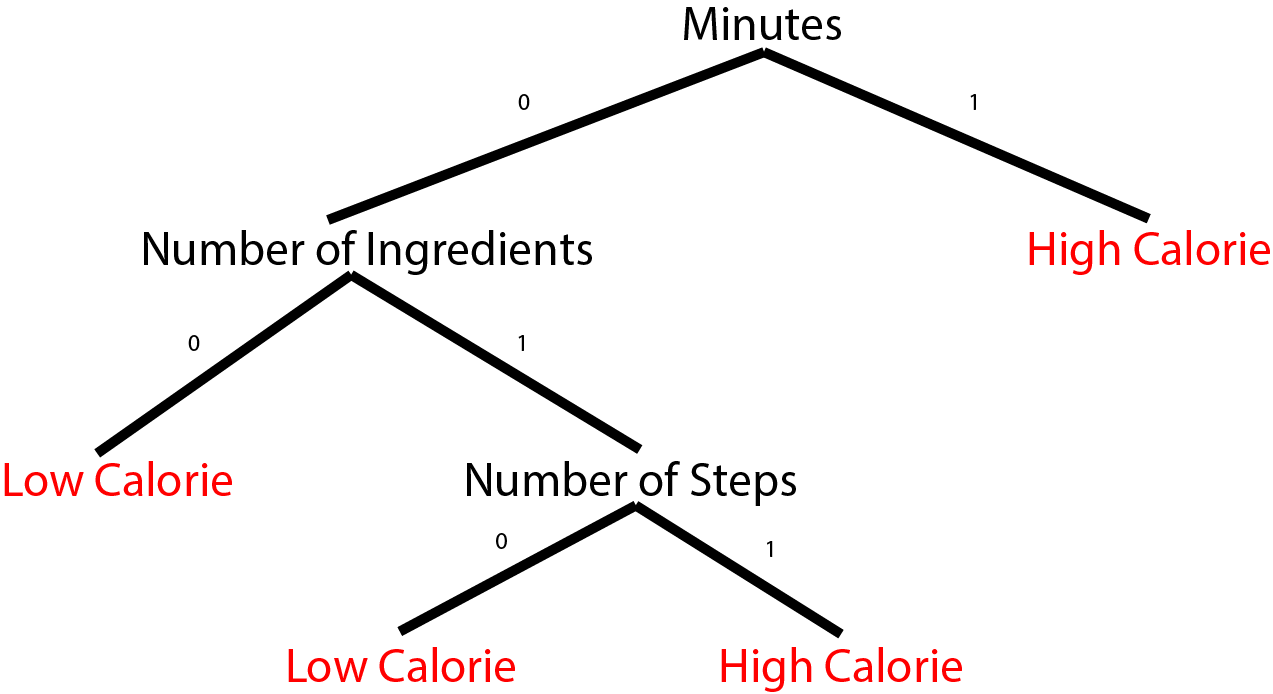
\includegraphics[width=\linewidth]{decisiontree.png}
\captionof{figure}{Visualization of generated decision tree}


\subsection{Recipe Recommendation}
For the task of Recipe Recommendation, we followed the approach outlined in "An Unsupervised Content-Based Article Recommendation System Using Natural Language Processing" by Renuka et al.\cite{RSArticle}. In doing so, we take a content-based approach to building as recommendation system, meaning that we create recommendations for recipes purely based on their features. The bulk of effort in this approach falls into two categories: feature engineering, and methodology to select similar articles.

Feature engineering is particularly important to us, because we are dealing with primarily text data. To featurize our text data, we first remove non-alphabetic characters. This is so that extraneous information like quantities or punctuation influence our recommendations. Next, we convert all text to lowercase to normalize all remaining words. Then we tokenize all words in the text and perform lemmatization on them. The lemmatization process further standardizes words by removing morphological affixes from the words. For example, "cookies" would become "cookie." Finally, each document is vectorized as a TF-IDF term matrix. This converts the text values to continuous values that describe frequency and the inter-document occurrence of words. Note that unlike Renuka et al., we did not perform Rake keyword extraction. We did this because we did not consider ngrams other than unigrams. In addition to the features extracted from the text, we also retain some key features like number of steps, nutritional information, number of minutes to cook recipe. While Renuka et al. did not include additional metadata features, we felt this metadata was an important factor people consider when comparing the similarity of recipes. Thus, it would be logical for a recommendation system to include these factors. At this point, we are ready to learn models to define similarity between recipes.

Renuka et al. outline three approaches for article recommendation: Cosine Similarity, KMeans Clustering, and Agglomerative Clustering. Each method encodes the similarity between documents, and thus falls under the category of content-based recommendation systems. Our Cosine Similarity approach simply iterates over all recipes and finds the top k recipes with lowest cosine distance. Our KMeans Clustering approach learns a KMeans model to assign centroids, then finds the top k closest recipes within the same cluster as the query recipe based on euclidean distance. Agglomerative Clustering takes the same approach, but using Agglomerative Clustering instead of KMeans. For both KMeans and Agglomerative Clustering we find the appropriate number of clusters by learning models with a different number of clusters, then plotting the within cluster sum of squared distances. An appropriate K is then selected from the resulting elbow plot. Additionally, due to the impracticality of training the Agglomerative Clustering algorithm on the entire dataset, a subset of only $1,000$ recipes were used to train the model. As seen in the elbow plots in Figures 1 and 2, the WC-SSD score begins to plateau after the number of clusters is $8$. Thus, $8$ was selected as the number of clusters for both KMeans and Agglomerative Clustering.

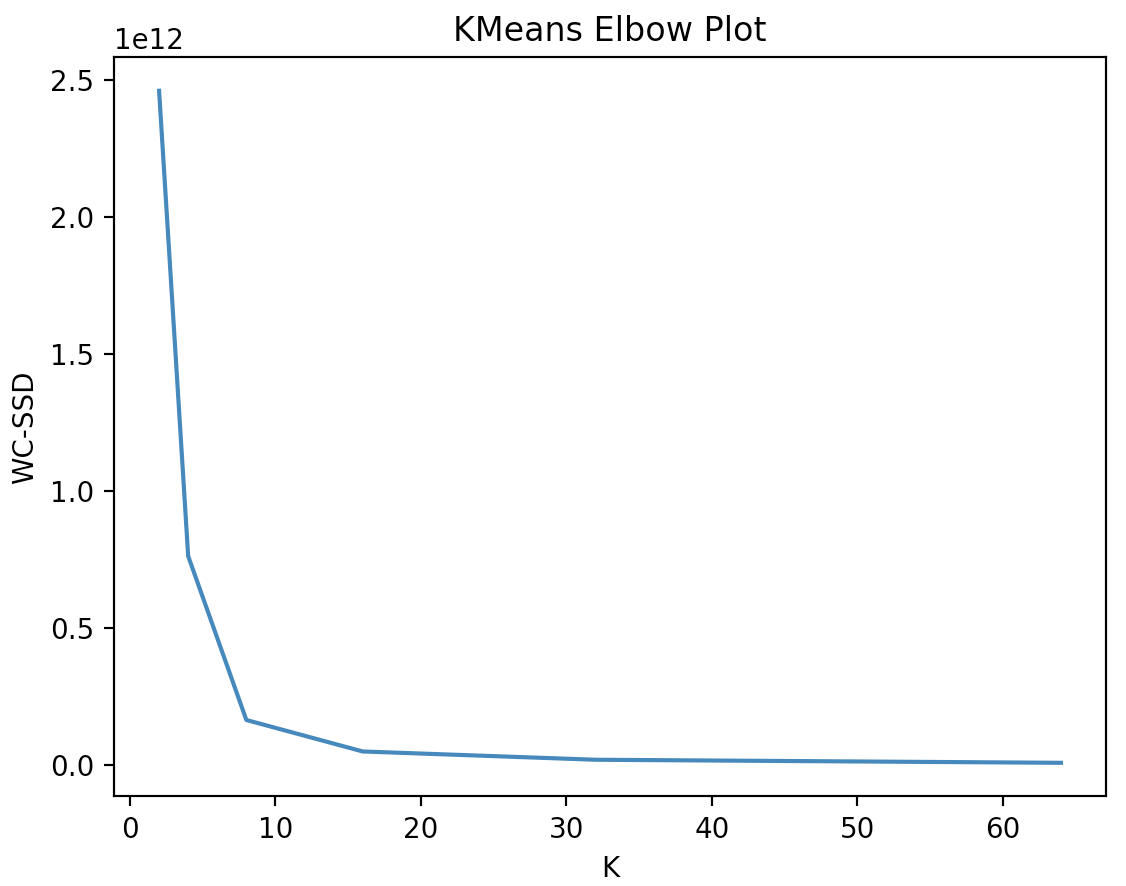
\includegraphics[width=\linewidth]{kmeansplot.png}
\captionof{figure}{KMeans Clustering Elbow Plot using Within Cluster-Sum of Squared Distances}

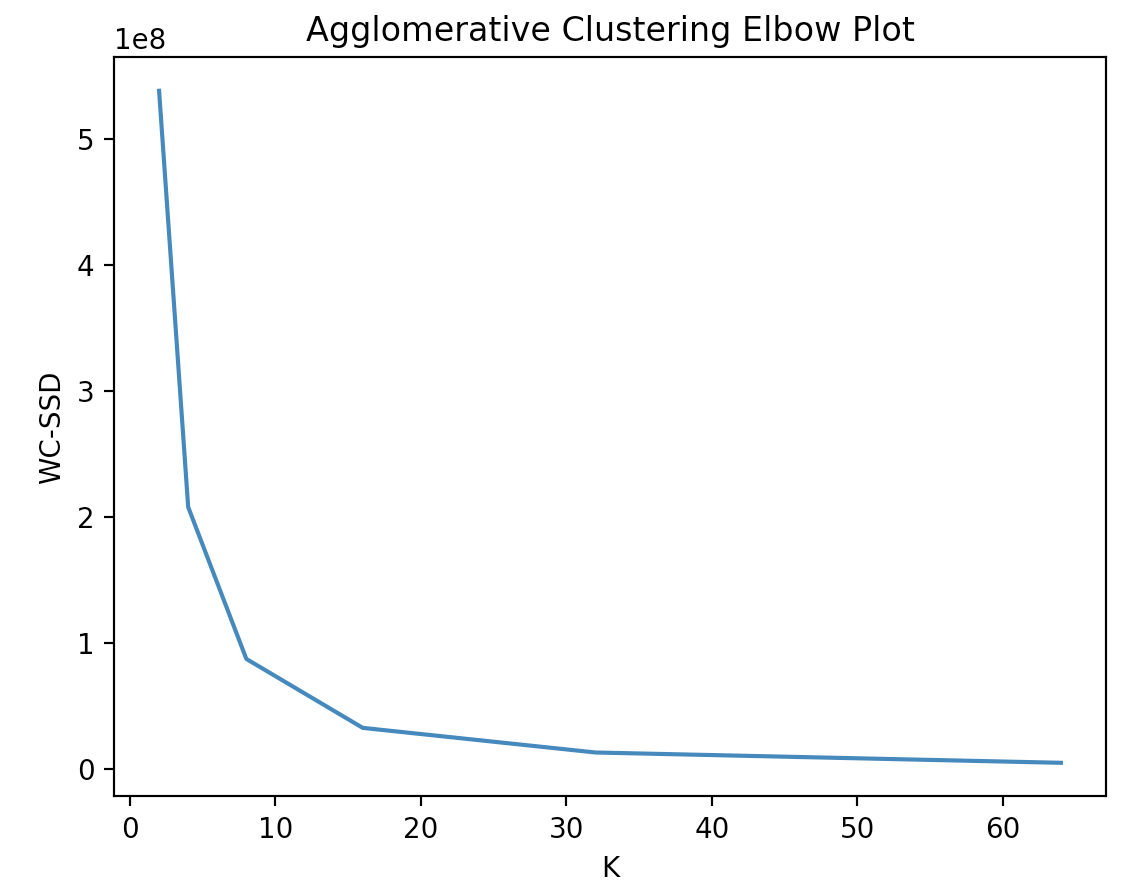
\includegraphics[width=\linewidth]{agglomerativeplot.png}
\captionof{figure}{Agglomerative Clustering Elbow Plot using Within Cluster-Sum of Squared Distances}

\subsection{Recipe Ingredient Prediction}
For the task of ingredient prediction, we sought to develop a model that captured the relationship among ingredients and with other recipe components. However, ingredients are an exceedingly rare feature with over ninety-nine percent of ingredients appearing is less than two percent of the recipes. Therefore, based on our initial data analysis and early modeling efforts working with all ingredients, we simplified to using only the 100 most common ingredients as prediction targets and features. Our ingredient prediction method consists of developing a model for each of the 100 ingredients. The first feature, used for all ingredients, was calorie level which had three levels (low, medium, high), each with similar frequency. The second feature was the number of ingredients. This represented the number of ingredients across all ingredients, not only the top 100. Finally, there was a one-hot encoding feature for each of the top 100 ingredients except the one currently being predicted. Imbalance was addressed by weighting examples so that recipes with ingredients had a total weight as those without; recipes with a specific ingredient were multiplied by the number of recipes with the ingredient divided by the number without the ingredient. Logloss was used as the training metric and for hyperparameter tuning. Parameters were chosen using grid search with five fold cross validation with the options described in table ~\ref{table:ingred_pred_param_table}; options were chosen based on initial, manual modeling experimentation.
\begin{table}[h]
\begin{tabular}{|c|p{3cm}|}
\hline Parameter Name & Assessed Values \\
\hline Number of Rounds & 50, 200 \\
\hline Regularization Constant & .05, .1, .2 \\
\hline Minimum Data Points per Leaf & 10, 25, 50 \\
\hline
\end{tabular}
\caption{Ingredient Prediction Hyperparameters}
\label{table:ingred_pred_param_table}
\end{table}
Data was split 80/20 into a training and validation set and a testing set. The testing set was only used for final evaluation discussed in the Performance section. The actual models were gradient boosting decision trees created using the lightGBM library developed by Ke et al.\cite{NIPS2017_6449f44a}.


\subsection{Cooking Duration Prediction}
The task of predicting the cooking duration involved predicting recipes as "short", "medium" and "long" based on how long it took to prepare. Using the number of minutes from the dataset, the samples were binned into three equal sized buckets. Recipes that took 20 minutes or fewer were marked as short, 20-40 minute recipes were marked as medium and recipes taking 40-80 minutes were marked as long. The Naive Bayes classifier offers a simple probabilistic model that allows us to infer the most probable class of unseen text. The model relies on a bold assumption that does not apply to natural language. Nonetheless, in practice, its performance is comparable to more sophisticated models.\cite{CDPNaiveBayes} The dataset was cleaned to remove tokens that may not contribute to the recipe duration and to limit the vocabulary size. For this, punctuation were removed, the text was lower-cased, stop-words were removed, and all words were replaced by its root form using the Porter stemmer.\cite{Porter1980AnAF} The recipes were vectorized using TF-IDF. For evaluation, the Macro F1-score was used on the test dataset with 5-fold cross-validation.

\subsection{Recipe Generation}
The goal of the recipe generation task was to learn a language model from the training dataset and to generate new recipes from the learned model. The simplest language model is the n-gram model. 80\% of the dataset was used for training. By setting the values of $n = 1$, $n = 2$ and $n = 3$, three language models were trained. There is no objective metric that can be used to evaluate the performance of this task. Perplexity is a measure of how well a model can predict a sample. The perplexity of each recipe in the test dataset was calculated and the mean of the values was recorded for each value of $n$. The recipes were generated by randomly picking the next token from the learned n-grams in such a way that the most frequent n-gram would be more likely to be picked. Finally, the generated recipes were manually verified. 

\section{Performance}
\subsection{Recipe Rating Prediction}
Performance of the K-Nearest Neighbor rating prediction model was poor, with the best accuracy achieved using an L2 distance function and all features. Given that 100 features were constructed using ingredients and title keywords, and the quantity of these features greatly outweighs the number of numerical features used in the model, KNN using only numerical features was explored as well.


\begin{table}[h]
\begin{tabular}{|c|p{3cm}|}
     \hline Model & Validation Accuracy  \\
     \hline KNN (L2 Norm, All Features) & 0.44 \\
     \hline KNN (L2 Norm, Numerical Features) & 0.41 \\
     \hline KNN (L1 Norm, All Features) & 0.43 \\
     \hline KNN (L1 Norm, Numerical Features) & 0.41 \\
     \hline Linear Regression (All Features) & 0.40 \\
     \hline 
\end{tabular}
\captionof{table}{Performance of KNN and Linear Regression}
\end{table}

This yielded a slight decrease in accuracy. The small difference in accuracy can be explained by the fact that the title keyword and ingredient vectors are sparse, and KNN does not generalize well to predict rating as a result. KNN with an L2 norm performed slightly better than with an L1 norm, which is contradictory to the observation of  Jain et. al. that L1 norm may be better suited for sparse vectors of text data. The poor performance of KNN on numerical features is inline with the observed correlation matrix, as correlation of rating and calories, minutes, steps, number of ingredients and nutrients are all below 0.05.

\subsection{Recipe Nutrition Prediction}
Overall, the accuracy of this section was surprisingly high when the simple model, the small amount of continuous features, and the low correlation between features are considered. The reasons why a more complex model was not used will be covered in the evaluation section.
Accuracy on the training dataset was 0.601866, and accuracy on the testing dataset was 0.596025. Thus, overfitting doesn't seem to have been a problem here, and the model performs consistently. Better performance could probably have been achieved had more relevant continuous attributes been present in the dataset. This small number of features also constrained what models were actually effective on the dataset.

\subsection{Recipe Recommendation}
Unlike most data mining tasks, recommendation systems cannot be easily scored quantitatively. Instead, we rely on manual analysis to see if the results are sound. Generally, we find our results align with the results of Renuka et al.. Cosine similarity produces precise recommendations, KMeans Clustering produces general recommendations, and Agglomerative Clustering produces recommendations based on broad categories.

As seen in table ~\ref{tab:cos_sim_kmeans}, cosine similarity appears to make recommendations more based on the presence of a few keywords, whereas KMeans' recommendations are more generalized and tend to match the same category as the original recipe. In table ~\ref{tab:agglom_cluster}, we see results for Agglomerative Clustering, and see that Agglomerative Clustering generally makes recommendations for other deserts, when given a desert as an input. However, Agglomerative Clustering appears to confuse asian salad as a desert. The likely cause of this is the inclusion of additional, non-textual features like cooking time. 
\begin{table}[h]
\begin{tabular}{|c|p{3cm}|p{3cm}|}
     \hline Ranking & Cosine Similarity & KMeans Clustering  \\
     \hline 1 & easiest creamed spinach & grilled artichoke and spinach dip with pita wedges \\
     \hline 2 & sour cream cheddar corn casserole & sweet corn and jalapeno dip \\
     \hline 3 & canadian cheese spinach dip & martha s scalloped mushrooms \\
     \hline 4 & turnips gratines & golden onion bake \\
     \hline 5 & the best brussels sprouts ever & broccoli and cheese to please \\
     \hline 
\end{tabular}
\captionof{table}{Top 5 recommendations for Cosine Similarity and KMeans Clustering for input "smoked salmon and cream cheese soup"}
\label{tab:cos_sim_kmeans}
\end{table}

\begin{table}[h]
\begin{tabular}{|c|p{6cm}|}
     \hline Ranking & Agglomerative Clustering  \\
     \hline 1 & pineapple sticky buns \\
     \hline 2 & asian salad \\
     \hline 3 & easy scones \\
     \hline 4 & christmas walnut raisin pinwheels \\
     \hline 5 & brownookie \\
     \hline
\end{tabular}
\captionof{table}{Top 5 recommendations for Agglomerative Clustering for input "pumpkin swirl pie"}
\label{tab:agglom_cluster}
\end{table}

Despite the promising results for each recommendation method, each method appears to confuse condiments, sweets, and drinks. For example, when given an input of "poppy seed fruited cole slaw", Cosine Similarity will output a recommendation of "honey mustard sauce" and "mango avocado margarita." We suspect the cause of this issue is the additional non-text based features such as cooking time, in addition to the use of similar language in recipes for these types of food. Logically this makes sense as both a condiment and a drink may only take a few minutes to prepare, and both involve similar words like "stir", "mix", and "poor." A solution may be to include the use of bigrams and trigrams in the featureset, however this will further complicate the feature space, and the generated trigrams may still not delinate between these types. Thus another solution would be to train a secondary model which classifies a recipe as being a sweet, condiment, or drink, then filtering recommendations based on the prediction of said model.

\subsection{Recipe Ingredient Prediction}
\begin{figure}[h]
    \centering
    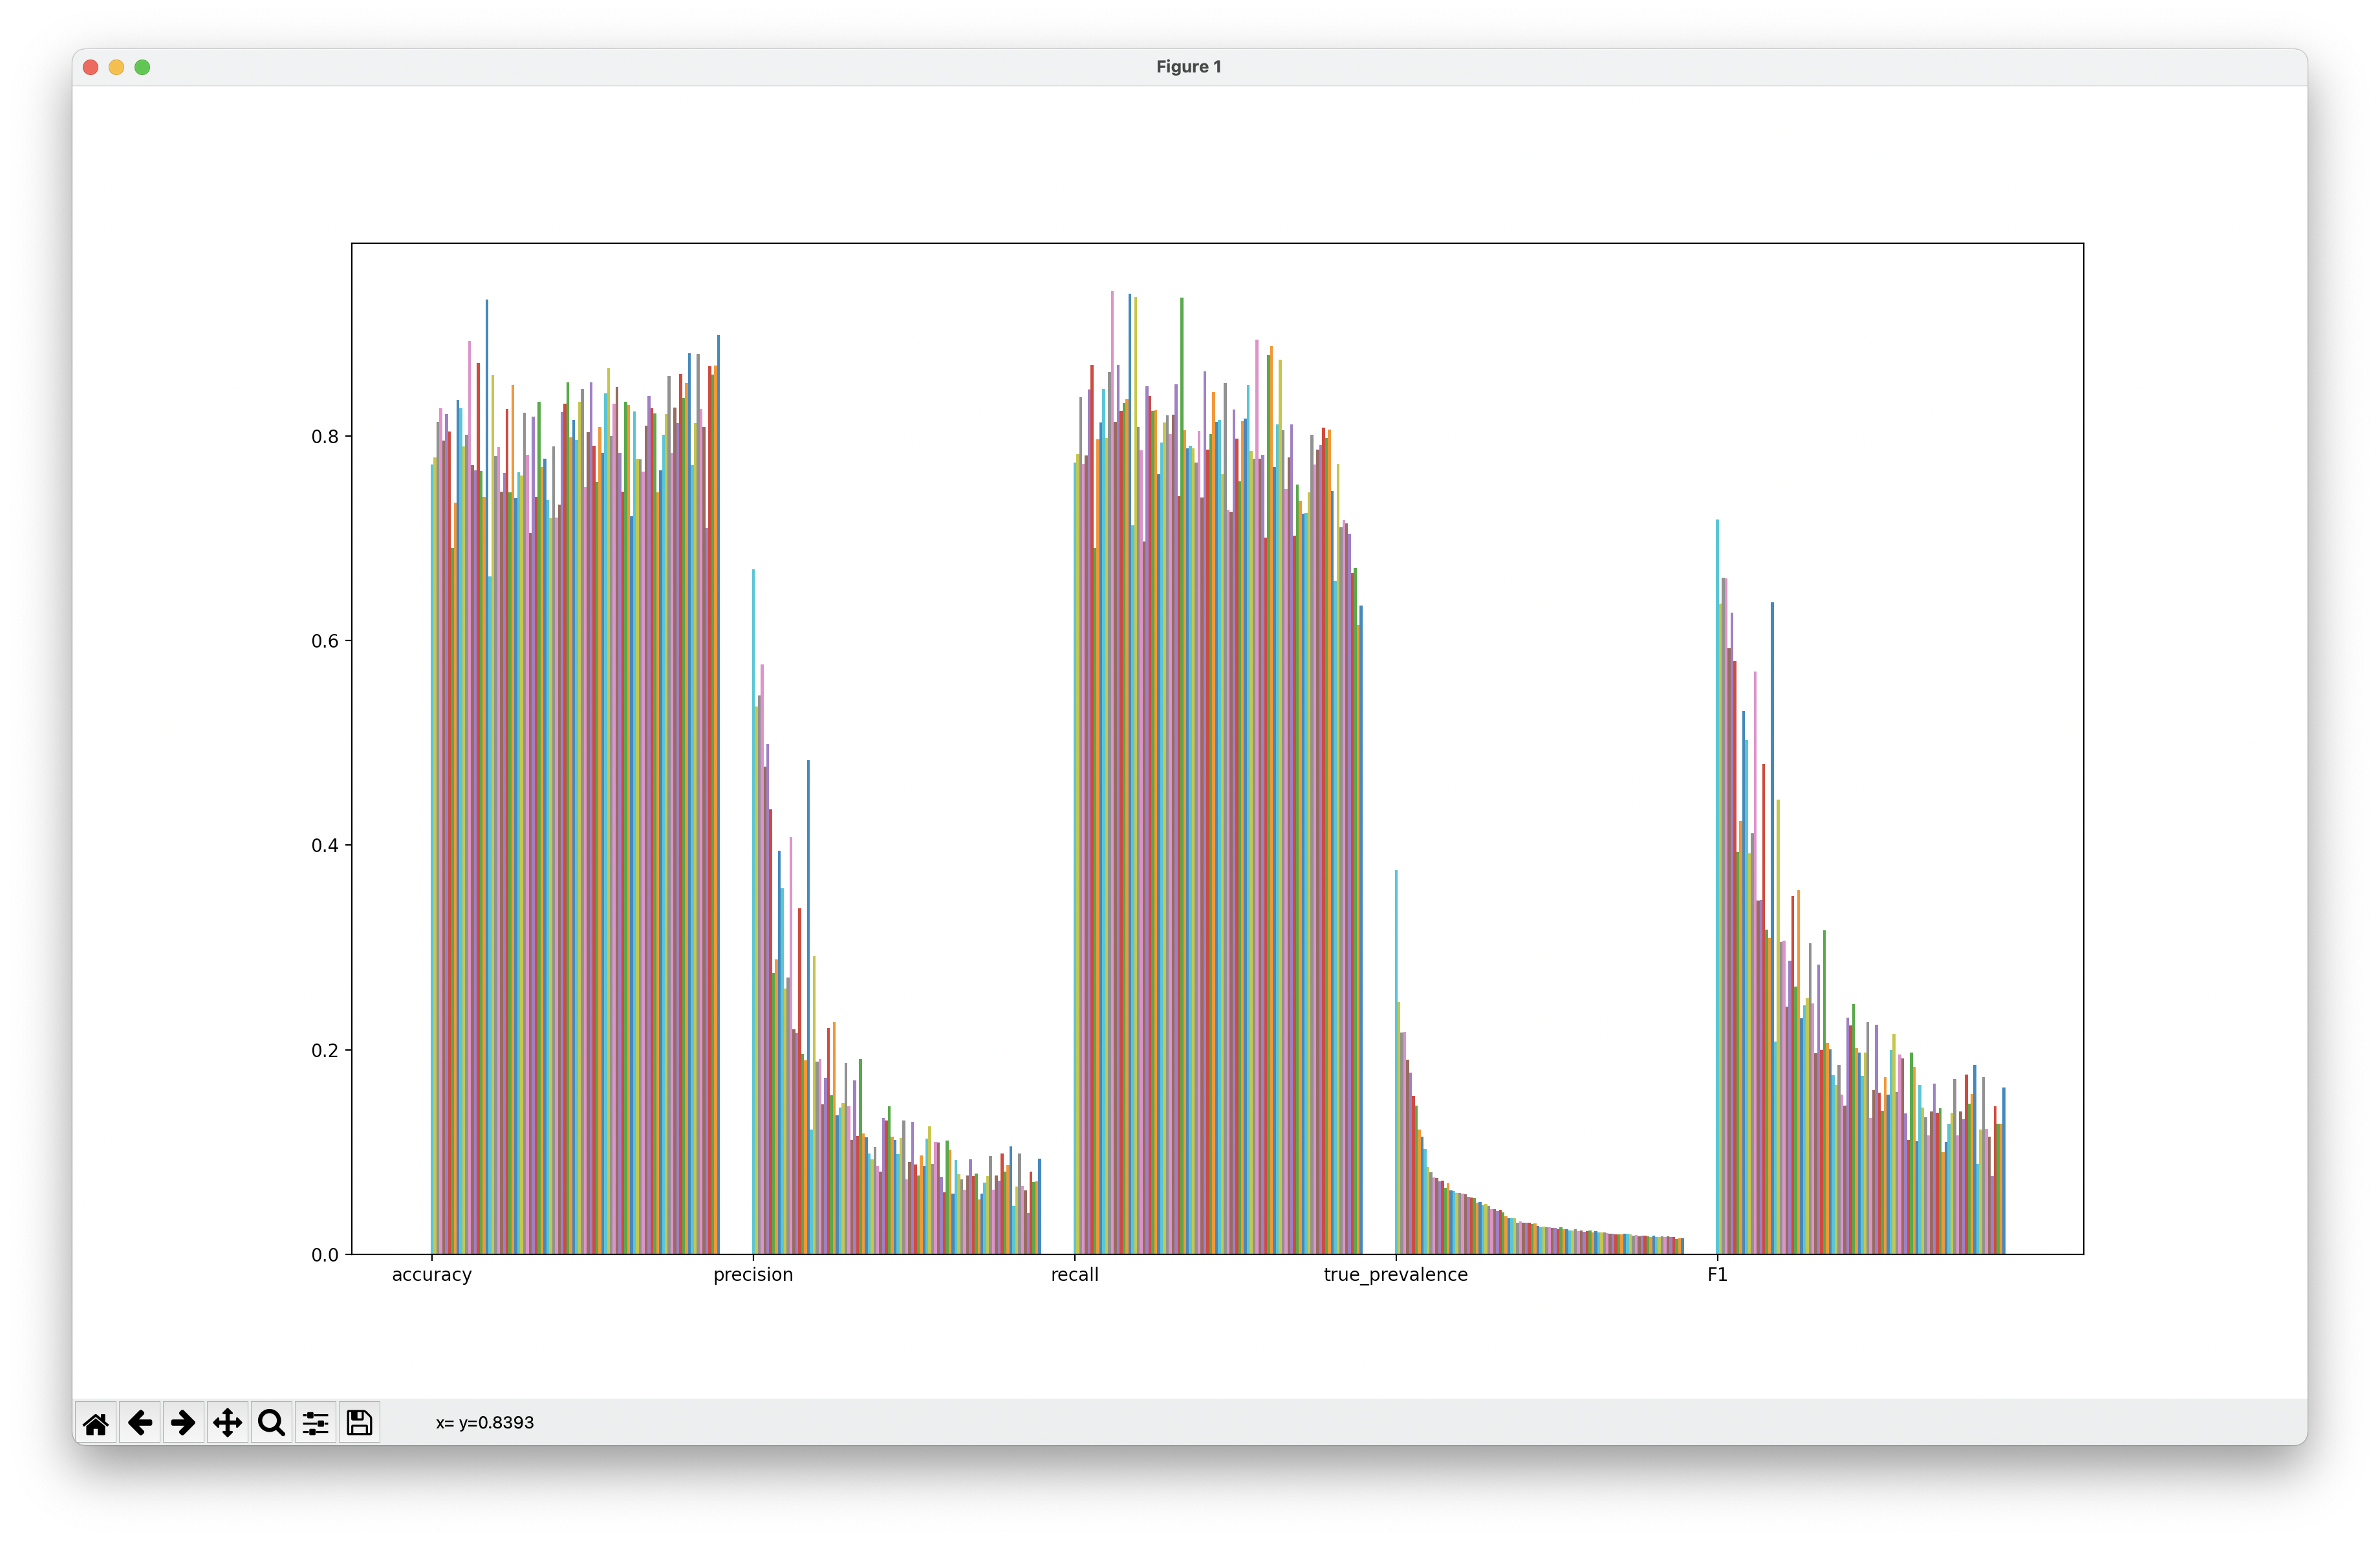
\includegraphics[width=\linewidth]{ingredient_pred_final.png}
    \caption{Ingredient prediction performance metrics (accuracy, precision, recall, true prevalence, F1 score)}
    \label{fig:ingred_pred_results}
\end{figure}
For evaluating ingredient prediction, we wanted to examine our model's ability to capture the value of interest, presence of a specific ingredient in a recipe, while maintaining reasonable performance in identifying recipes which do not contain a specific ingredient. Thus we evaluated each model on accuracy, precision, and recall (as well as F1 score) versus the true prevalence of an ingredient. Thus, we can capture if our model is able to out-perform a naive guess as to whether a recipe has an ingredient and we can also assess performance versus references. Lee et al. do achieve a higher F1 score for their ingredient prediction models (in the .7 range versus our roughly ~.1 to .7 range) \cite{NLPRecipeGPT}. However a direct comparison is difficult as their feature set is different including preparation steps and recipe title, the latter of which may include ingredients names in it and their data set is more than five times larger; on the other hand, they do not exclude rare ingredients from analysis. Performance versus a naive prediction is significantly easier to classify as out model has precision roughly 50-1000 percent better than the true prevalence while maintaining an overall accuracy over 64 percent (and generally, around 75 percent) for every ingredient. Recall is also always in excess of 60 percent. For specific values for each ingredient please see figure ~\ref{fig:ingred_pred_results}. Generally, the model is able to identify a subset of recipes which are far more likely to have an ingredient than the original population. Performance was noticeably better on ingredients with a higher true prevalence (see sections 2, 4, and 5 of figure ~\ref{fig:ingred_pred_results}). However, accuracy and recall (sections 1 and 3, respectively) remained high despite true prevalence.




\subsection{Cooking Duration Prediction}
\begin{figure}[h]
    \centering
    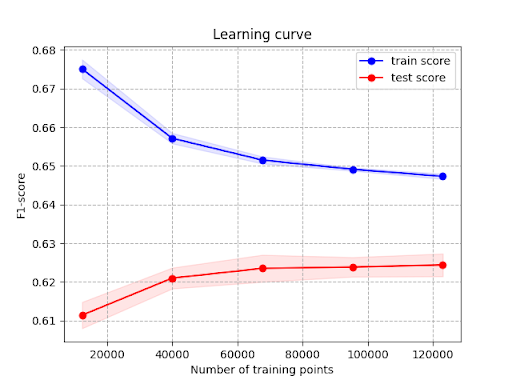
\includegraphics[width=\linewidth]{cooking_duration_learning_curve.png}
    \caption{Learning curve for predicting cooking duration with 5-fold cross-validation)}
    \label{fig:cooking_duration_learning_curve}
\end{figure}
\begin{table}[h]
\begin{tabular}{|c c c c|}
    \hline Class & Precision & Recall & F1-score\\
    \hline\hline Short & 0.7383 & 0.5975 & 0.6605 \\
    \hline Medium & 0.5070 & 0.6346 & 0.5637 \\
    \hline Long & 0.6613 & 0.6122 & 0.6358 \\
    \hline
\end{tabular}
\caption{Cooking duration results}
\label{tab:cooking_duration_results}
\end{table}
The Macro-F1 score of the trained classifier was 0.62, which is better than 0.33 that one would expect from a random guess. Figure \ref{fig:cooking_duration_learning_curve} is the learning curve for the same. The model seems to be able to reach the optimal test accuracy after training with half the training set. The confusion matrix in Figure \ref{fig:cooking_duration_confusion_matrix} was constructed from the test dataset. The model seemed to perform well for the short and the long recipes but was not as precise for the medium recipes. This is probably because the tokens present in this class would be spread out in the other two classes as well. To analyze this claim, we constructed Table \ref{tab:cooking_duration_conditional_probability}. The table lists the highest conditional probabilities it has learned for each class. The highest values for the medium class is less than that of the other two classes. Another insight from the table is the tokens itself in the class. It seems like the tokens in the short class must belong to recipes that are juices, milkshakes and sandwiches. On the other hand, tokens in the long class seem to belong to recipes that involve baking. This should have been obvious had we read through recipes with intent of preparing it. Nonetheless, it is an interesting insight that we got after training the classifier.

\begin{figure}[h]
    \centering
    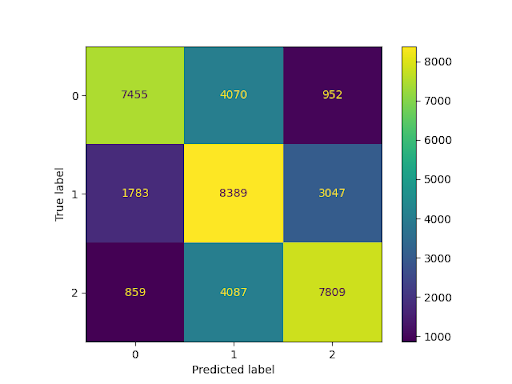
\includegraphics[width=\linewidth]{cooking_duration_confusion_matrix.png}
    \caption{Confusion matrix of the cooking duration prediction model}
    \label{fig:cooking_duration_confusion_matrix}
\end{figure}

% Note: the typos in this table are not typos. These are the tokens in the model's vocabulary after stemming the words in the recipe during pre-processing%
\begin{table}[h]
\begin{tabular}{|c c c|}
    \hline Short & Medium & Long\\
    \hline\hline glass (0.791) & muffin (0.657) & 40 (0.898) \\
    \hline ice (0.714) & 20 (0.531) & loaf (0.805) \\
    \hline blender (0.707) & patti (0.521) & 45 (0.779) \\
    \hline shake (0.681) & tin (0.514) & casserol (0.676) \\
    \hline lettuc (0.628) & degre (0.498) & insert (0.659) \\
    \hline
\end{tabular}
\caption{Top 5 learned probabilities of frequent (>5000) tokens in each class}
\label{tab:cooking_duration_conditional_probability}
\end{table}

\subsection{Recipe Generation}
The language model built using n-grams performed better while increasing the value of $n$. With $n = 1$, the generated text did not make sense. With $n = 2$, the model sometimes returned some coherent phrases but was mostly random. The model with $n = 3$, gave out many more coherent phrases. In some cases, the trigram-based model was grammatically correct. We can see this improvement from the decreasing value of perplexity in Table \ref{tab:recipe_generation_perplexity}. Few of the generated recipes are listed in Table \ref{tab:recipe_generation_samples}. Setting $n = 4$ increased the vocabulary size drastically and therefore was not practical to implement. The trigram-based model performed the best. However, the quality of the generated recipe is still subjective. It would require sophisticated metrics and domain knowledge to evaluate them correctly. 

\begin{table}[]
    \centering
    \begin{tabular}{|c|c|}
        \hline n & Perplexity \\
        \hline\hline 1 (Unigram) & 486.71\\
        \hline 2 (Bigram) & 57.92\\
        \hline 3 (Trigram) & 14.36\\
        \hline
    \end{tabular}
    \caption{Perplexity of the n-gram based recipe generation models}
    \label{tab:recipe_generation_perplexity}
\end{table}

\begin{table}[]
    \centering
    \begin{tabular}{|p{8cm}|}
        \hline Generated Recipes \\
        \hline\hline Wine to the pot take a large sauce pan and set on paper towels  and drain off all but 2 tablespoons olive oil\\
        \hline Eggs to flour mixture and coat bottom of a golf ball and put mixture in a large bowl add wine lemon pepper rosemary and black\\
        \hline Stir frequently until soft peaks form and the water bring to boil cover and cook until meat is very tender season to taste fill the\\
        \hline
    \end{tabular}
    \caption{Recipes generated by the trigram model by limiting the recipe to 25 words}
    \label{tab:recipe_generation_samples}
\end{table}


\section{Insights}
Perhaps the most difficult part of the project was working with textual data. Unlike standard datasets where the majority of the features are discrete or continuous, textual data requires a significant amount of pre-processing into features before it can be effectively applied. This process also requires a lot of experimentation to find the right parameters to create these features from. Even if the correct set of parameters are found, the feature space for these newly created features is generally very sparse as the features tend to be text encodings. Data exploration was key for indentifying subproblems with moderate sparseness (presence of the target feature in at least one percent of samples) which can be partially addressed by weighting features to still achieve meaningful results. However, to fully overcome this sparseness, or to deal with the vast majority of features with frequencies below one percent of sample, either a significant amount of data is required for strong results, more complex feature extraction must be used, or more complex models must be deployed. We suspect this is why existing recipe generation models like RecipeGPT\cite{NLPRecipeGPT} and RecipeGM\cite{NLPRecipeGM} use highly sophisticated models.

Further, as discussed by Reusch et al.\cite{NLPRecipeGM}, evaluation of textual output, specifically recipes, from models is quite difficult. This is because recipes are subjectively scored by humans and each human has their own preference. Thus determining the quality of a recipe recommendation or recipe generation requires prior knowledge of the interaction of food ingredients as well as the user's preferences.

Lastly, we found that the performance of our models suffered when predicting continuous attributes. Instead, we found that the performance of our models significantly increased when we discretized the target attribute and applied a classification model to the new feature set. This is likely due to non-linear interactions between features, possibly caused by the truncation of quantities during pre-processing. The importance of exploratory data analysis was also shown for discretization, as not accounting for skew led to useless results with unrealistically high accuracies, as the feature being predicted was discretized highly unequally into its bins. Thus, feature engineering is a powerful tool that must be used carefully.
\section{Evaluation}
\subsection{Recipe Rating Prediction}
Predictions of rating with accuracy of below 50 percent suggest that prediction of average rating based on the outlined models is ineffective. Prediction of rating for each individual interacting with the recipe dataset may yield better results. However, with an average of 5 interactions per active user in this dataset, there is an insufficient quantity of observations to make user-specific recipe rating predictions. Using a larger data set of interactions may yield user-specific rating predictions that are significantly more accurate. However, the sparsity of the ingredient and keyword vectors are challenges that may hinder model performance.
\subsection{Recipe Nutrition Prediction}
The accuracy of the decision tree used for predicting calorie values, which was consistently around 60\%, was surprisingly high given the simple model and the limited number of features used. In fact, the small amount of discretizable features mean that more complex ensemble models like bagged trees or random forests are completely wasted, as there is simply not enough variation to warrant them. The learning curve of a random forest generated using the same method with tree number as the independent variable was essentially a straight line at 0.60 accuracy, leading to the usage of a simpler model. Nevertheless, this task was significantly better than just a random guess, so we are quite happy with the results. Thus, this task can be viewed as a demonstration of the power of simple models given adequate feature engineering.
\subsection{Recipe Recommendation}
Despite the relative simplicity of the features used for model training, the recommendation models generally made sensible recommendations. However, the models often confused classes of items that used similar preparation or cooking methods, like drinks and condiments. Cosine Similarity performed the best at making precise recommendations, with both the KMeans and Agglomerative Clustering methods coming in second, performing well at general recommendations. Future improvements to the recommendation system include the application of collaborative filtering using user rating information, use of hybrid recommendation systems, further including recipe metadata to improve model performance, and the incorporation of auxiliary models into a hybrid system to further distinguish between classes of recipes and thus provide better recommendations.
\subsection{Recipe Ingredient Prediction}
With the vast majority of ingredients predicted with a precision of less than 50 percent, cooking using ingredients generated by our model may not be enjoyable. However, by creating a narrower subset of recipes which may have an ingredient it can still be useful for our motivation of assisting chefs with recipe creation by cutting down on the number of considerations when creating new versions of recipes. In addition, evaluation of our model cannot capture what we term correct mistakes. This category includes generating an existing, valid recipe which is different than the one under consideration. It also includes tasty, but currently unknown recipes which were not in our dataset where the model adds an ingredient to a recipe where it would be beneficial but had not previously been tried. Both categories are also useful for experimenting chefs, and, thus, the true utility of our model may be higher than our metrics can capture.
\subsection{Cooking Duration Prediction}
The Macro-F1 score of the learned model was much better than a random guess but slightly short of our goal of 0.7 that was observed in comparable tasks during literature review. The performance can be improved by modifying the feature selection process and using a score-based strategy for probabilities instead of relying solely on the frequency.\cite{CDPImproveNaiveBayes} The text classification problem does not follow the naive assumption. Text data is context-sensitive. However, the fact that a simple classifier could perform satisfactorily demonstrates the capabilities of such simple models.
\subsection{Recipe Generation}
The initial goal for this task was to see recipe generation was possible. By manually reading through the output, the results were satisfactory. Nonetheless, a better model could be learnt by reusing pre-trained language models and retraining them on our dataset. There are also some techniques to train n-gram based language models for larger values of $n$.\cite{RG_GrowingNGramModels} From the trend observed in the performance of the model, a better perplexity can be expected.
\section{Contributions}

\begin{itemize}
    \item 
    Reece Jones performed part of the literature review, took an attempt at the nutrition prediction model, implemented the recipe recommendation models, and wrote large parts of the Proposal, Midterm Report, and Final Report.
    
    \item
    Eli Silkov performed the exploratory data analysis, performed modelling exploration, implemented rating predictions, and contributed to all writings and presentations.
    
    \item
    Nathan Merz identified the dataset used in our modeling and exploration, performed intial modeling exploration, implemented the ingredient prediction modeling, and contributed to all writings and the presentation.
    
    \item
    Patrick Li performed part of the literature review, implemented the nutrition prediction model, and contributed significant parts of the Proposal, Midterm Report, and Final Report.
    
    \item
    Varun Vora performed a part of the exploratory data analysis, implemented cooking duration prediction model, implemented the recipe prediction model and contributed to the corresponding sections in the final presentation and report.
\end{itemize}

\section{Conclusion}
For our project, we implemented six tasks that all relied on varying data mining techniques. We predicted recipe ratings, predicted recipe ingredients, predicted nutritional information of recipes, predicted the cooking time of recipes, generated recipe recommendations, and generated novel recipes. Through each task we gained a better understanding of how data mining techniques can be used to solve complex problems, and how we can further use these techniques to produce better results. We also learned the drawbacks of some techniques, and how these drawbacks can be overcome by feature engineering, parameter tuning, or the selection of a different model.

The project code is accessible here: \url{https://github.com/ReeceJones/CS573-Project}.

%
%%
%% The acknowledgments section is defined using the "acks" environment
%% (and NOT an unnumbered section). This ensures the proper
%% identification of the section in the article metadata, and the
%% consistent spelling of the heading.
\begin{acks}
Idea consultation: Altug Gemalmaz\\
Data source: Shuyang Li
\end{acks}

%%
%% The next two lines define the bibliography style to be used, and
%% the bibliography file.
\bibliographystyle{ACM-Reference-Format}
\bibliography{midterm-refs}
%% Shuyang Li, “Food.com Recipes and Interactions.” Kaggle, 2019, doi: 10.34740/KAGGLE/DSV/783630.

%%
%% If your work has an appendix, this is the place to put it.
%\appendix

\end{document}
\endinput
%%
%% End of file `sample-authordraft.tex'.
